% Options for packages loaded elsewhere
\PassOptionsToPackage{unicode}{hyperref}
\PassOptionsToPackage{hyphens}{url}
\PassOptionsToPackage{dvipsnames,svgnames,x11names}{xcolor}
%
\documentclass[
  letterpaper,
  DIV=11,
  numbers=noendperiod]{scrreprt}

\usepackage{amsmath,amssymb}
\usepackage{iftex}
\ifPDFTeX
  \usepackage[T1]{fontenc}
  \usepackage[utf8]{inputenc}
  \usepackage{textcomp} % provide euro and other symbols
\else % if luatex or xetex
  \usepackage{unicode-math}
  \defaultfontfeatures{Scale=MatchLowercase}
  \defaultfontfeatures[\rmfamily]{Ligatures=TeX,Scale=1}
\fi
\usepackage{lmodern}
\ifPDFTeX\else  
    % xetex/luatex font selection
\fi
% Use upquote if available, for straight quotes in verbatim environments
\IfFileExists{upquote.sty}{\usepackage{upquote}}{}
\IfFileExists{microtype.sty}{% use microtype if available
  \usepackage[]{microtype}
  \UseMicrotypeSet[protrusion]{basicmath} % disable protrusion for tt fonts
}{}
\makeatletter
\@ifundefined{KOMAClassName}{% if non-KOMA class
  \IfFileExists{parskip.sty}{%
    \usepackage{parskip}
  }{% else
    \setlength{\parindent}{0pt}
    \setlength{\parskip}{6pt plus 2pt minus 1pt}}
}{% if KOMA class
  \KOMAoptions{parskip=half}}
\makeatother
\usepackage{xcolor}
\usepackage[heightrounded]{geometry}
\setlength{\emergencystretch}{3em} % prevent overfull lines
\setcounter{secnumdepth}{-\maxdimen} % remove section numbering
% Make \paragraph and \subparagraph free-standing
\ifx\paragraph\undefined\else
  \let\oldparagraph\paragraph
  \renewcommand{\paragraph}[1]{\oldparagraph{#1}\mbox{}}
\fi
\ifx\subparagraph\undefined\else
  \let\oldsubparagraph\subparagraph
  \renewcommand{\subparagraph}[1]{\oldsubparagraph{#1}\mbox{}}
\fi


\providecommand{\tightlist}{%
  \setlength{\itemsep}{0pt}\setlength{\parskip}{0pt}}\usepackage{longtable,booktabs,array}
\usepackage{calc} % for calculating minipage widths
% Correct order of tables after \paragraph or \subparagraph
\usepackage{etoolbox}
\makeatletter
\patchcmd\longtable{\par}{\if@noskipsec\mbox{}\fi\par}{}{}
\makeatother
% Allow footnotes in longtable head/foot
\IfFileExists{footnotehyper.sty}{\usepackage{footnotehyper}}{\usepackage{footnote}}
\makesavenoteenv{longtable}
\usepackage{graphicx}
\makeatletter
\def\maxwidth{\ifdim\Gin@nat@width>\linewidth\linewidth\else\Gin@nat@width\fi}
\def\maxheight{\ifdim\Gin@nat@height>\textheight\textheight\else\Gin@nat@height\fi}
\makeatother
% Scale images if necessary, so that they will not overflow the page
% margins by default, and it is still possible to overwrite the defaults
% using explicit options in \includegraphics[width, height, ...]{}
\setkeys{Gin}{width=\maxwidth,height=\maxheight,keepaspectratio}
% Set default figure placement to htbp
\makeatletter
\def\fps@figure{htbp}
\makeatother

\usepackage{fvextra}
\DefineVerbatimEnvironment{Highlighting}{Verbatim}{breaklines,commandchars=\\\{\}}
\KOMAoption{captions}{tableheading}
\makeatletter
\@ifpackageloaded{tcolorbox}{}{\usepackage[skins,breakable]{tcolorbox}}
\@ifpackageloaded{fontawesome5}{}{\usepackage{fontawesome5}}
\definecolor{quarto-callout-color}{HTML}{909090}
\definecolor{quarto-callout-note-color}{HTML}{0758E5}
\definecolor{quarto-callout-important-color}{HTML}{CC1914}
\definecolor{quarto-callout-warning-color}{HTML}{EB9113}
\definecolor{quarto-callout-tip-color}{HTML}{00A047}
\definecolor{quarto-callout-caution-color}{HTML}{FC5300}
\definecolor{quarto-callout-color-frame}{HTML}{acacac}
\definecolor{quarto-callout-note-color-frame}{HTML}{4582ec}
\definecolor{quarto-callout-important-color-frame}{HTML}{d9534f}
\definecolor{quarto-callout-warning-color-frame}{HTML}{f0ad4e}
\definecolor{quarto-callout-tip-color-frame}{HTML}{02b875}
\definecolor{quarto-callout-caution-color-frame}{HTML}{fd7e14}
\makeatother
\makeatletter
\@ifpackageloaded{caption}{}{\usepackage{caption}}
\AtBeginDocument{%
\ifdefined\contentsname
  \renewcommand*\contentsname{Table of contents}
\else
  \newcommand\contentsname{Table of contents}
\fi
\ifdefined\listfigurename
  \renewcommand*\listfigurename{List of Figures}
\else
  \newcommand\listfigurename{List of Figures}
\fi
\ifdefined\listtablename
  \renewcommand*\listtablename{List of Tables}
\else
  \newcommand\listtablename{List of Tables}
\fi
\ifdefined\figurename
  \renewcommand*\figurename{Figure}
\else
  \newcommand\figurename{Figure}
\fi
\ifdefined\tablename
  \renewcommand*\tablename{Table}
\else
  \newcommand\tablename{Table}
\fi
}
\@ifpackageloaded{float}{}{\usepackage{float}}
\floatstyle{ruled}
\@ifundefined{c@chapter}{\newfloat{codelisting}{h}{lop}}{\newfloat{codelisting}{h}{lop}[chapter]}
\floatname{codelisting}{Listing}
\newcommand*\listoflistings{\listof{codelisting}{List of Listings}}
\makeatother
\makeatletter
\makeatother
\makeatletter
\@ifpackageloaded{caption}{}{\usepackage{caption}}
\@ifpackageloaded{subcaption}{}{\usepackage{subcaption}}
\makeatother
\makeatletter
\@ifpackageloaded{tcolorbox}{}{\usepackage[skins,breakable]{tcolorbox}}
\makeatother
\makeatletter
\@ifundefined{shadecolor}{\definecolor{shadecolor}{rgb}{.97, .97, .97}}{}
\makeatother
\makeatletter
\@ifundefined{codebgcolor}{\definecolor{codebgcolor}{HTML}{D3D3D3}}{}
\makeatother
\makeatletter
\ifdefined\Shaded\renewenvironment{Shaded}{\begin{tcolorbox}[colback={codebgcolor}, sharp corners, enhanced, boxrule=0pt, frame hidden, breakable]}{\end{tcolorbox}}\fi
\makeatother
\ifLuaTeX
  \usepackage{selnolig}  % disable illegal ligatures
\fi
\usepackage{bookmark}

\IfFileExists{xurl.sty}{\usepackage{xurl}}{} % add URL line breaks if available
\urlstyle{same} % disable monospaced font for URLs
\hypersetup{
  colorlinks=true,
  linkcolor={blue},
  filecolor={Maroon},
  citecolor={Blue},
  urlcolor={Blue},
  pdfcreator={LaTeX via pandoc}}

\author{}
\date{}

\begin{document}

\RecustomVerbatimEnvironment{verbatim}{Verbatim}{
  showspaces = false,
  showtabs = false,
  breaksymbolleft={},
  breaklines
}

\renewcommand*\contentsname{Table of contents}
{
\hypersetup{linkcolor=}
\setcounter{tocdepth}{1}
\tableofcontents
}
\section{HPC introduction}\label{hpc-introduction}

If you work at IBED you can get access to the Crunchomics HPC, the
Genomics Compute Environment for SILS and IBED. If you need access to
Crunchomics, send an email to Wim de Leeuw
\href{mailto:w.c.deleeuw@uva.nl}{\nolinkurl{w.c.deleeuw@uva.nl}} to get
an account set up by giving him your UvA netID.

Using an HPC works a bit differently than running jobs on your computer,
below you find a simplified schematic:

\begin{center}
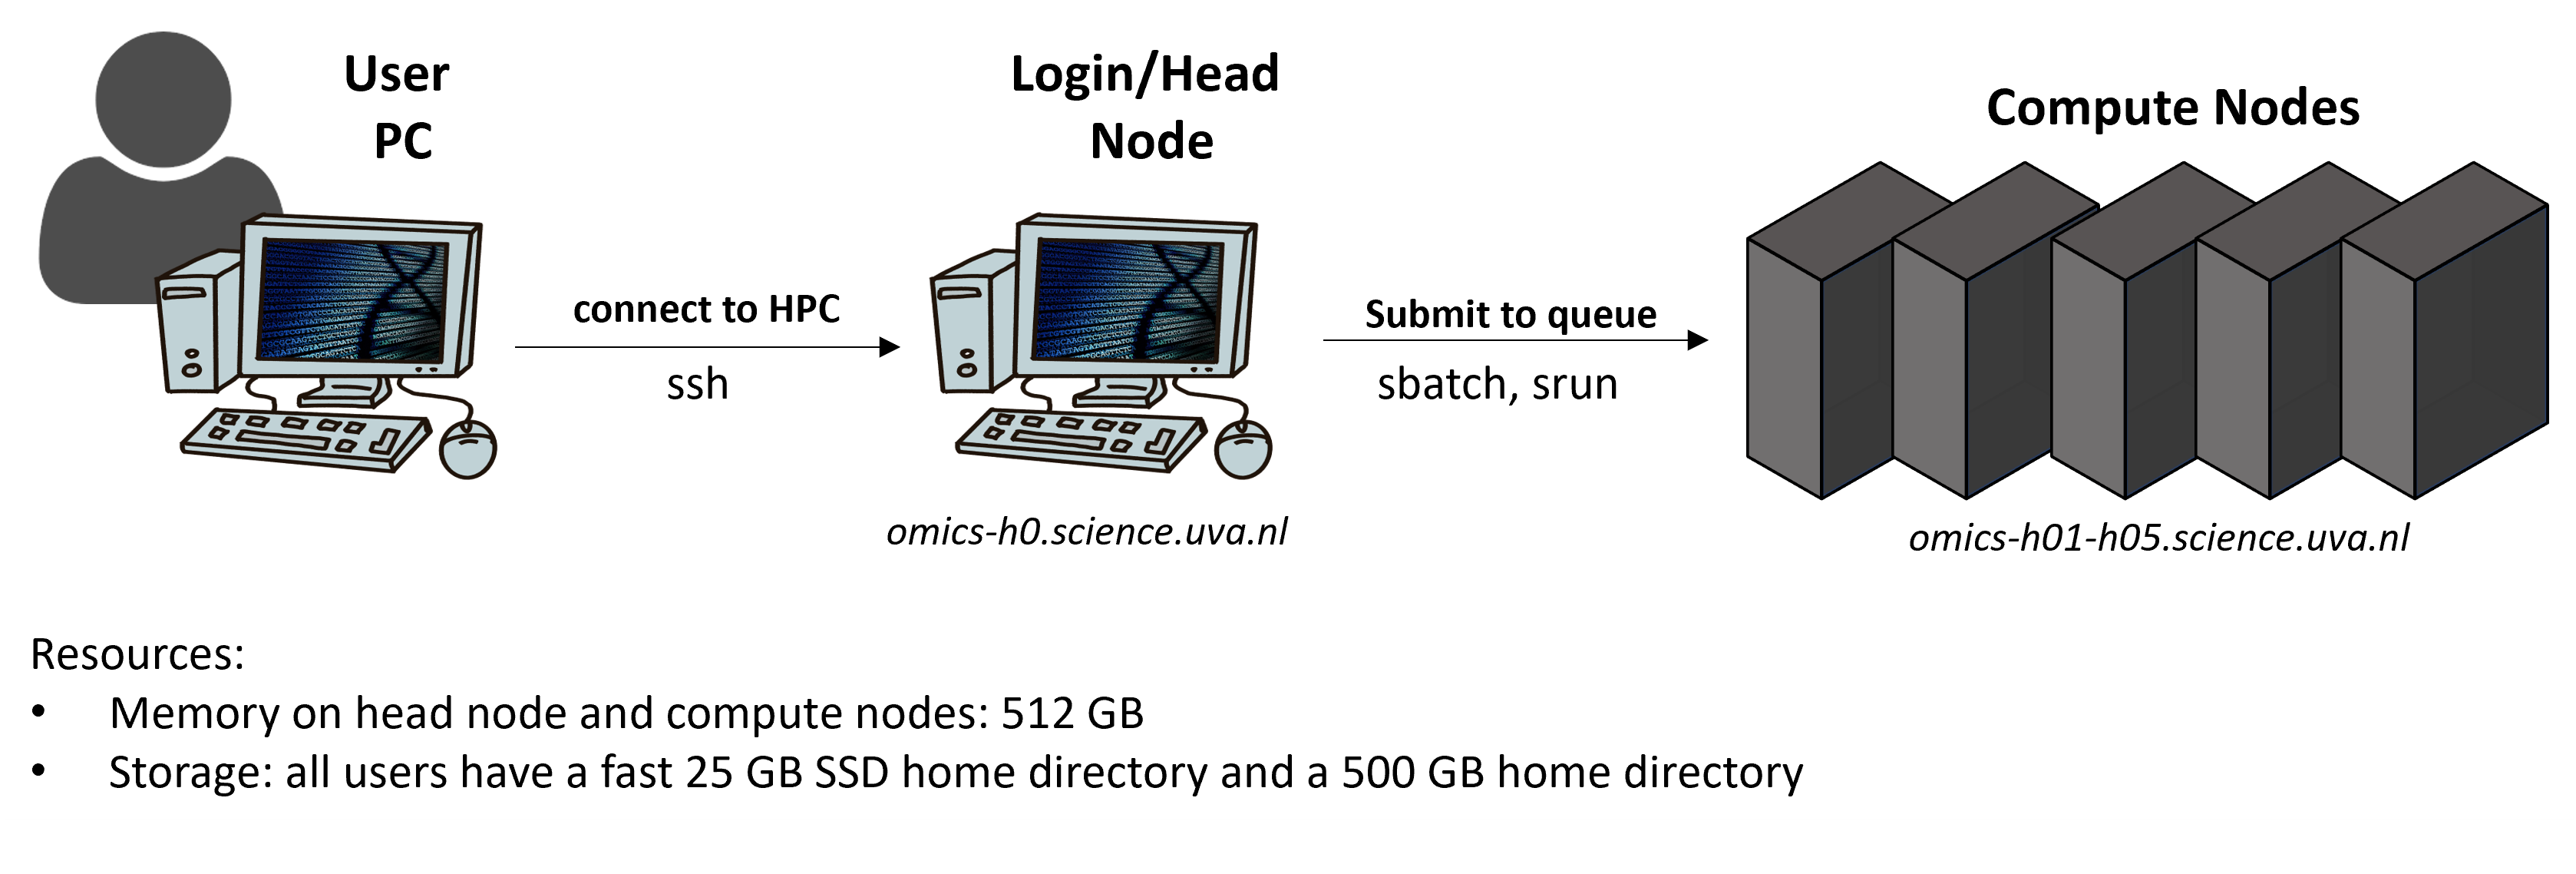
\includegraphics[width=0.7\textwidth,height=\textheight]{../img/crunchomics1.png}
\end{center}

Very briefly, you can log into an HPC onto a login node. The purpose of
a \textbf{login node}, sometimes also called head node, is to prepare to
run a program (e.g., moving and editing files as well as compiling and
preparing a job script). You then submit a job script from the head to
the compute nodes via Slurm. The \textbf{compute nodes} are used to
actually run a program and \textbf{Slurm} is an open-source workload
manager/scheduler that is used on many big HPCs. Slurm has three key
functions:

\begin{itemize}
\tightlist
\item
  provide the users access to the resources on the compute nodes for a
  certain amount of time to perform any computation
\item
  provide a framework to start, execute, and check the work on the set
  of allocated compute nodes
\item
  mange the queue of submitted jobs based on the availability of
  resources
\end{itemize}

\begin{tcolorbox}[enhanced jigsaw, opacityback=0, coltitle=black, titlerule=0mm, colframe=quarto-callout-important-color-frame, rightrule=.15mm, bottomrule=.15mm, arc=.35mm, leftrule=.75mm, colbacktitle=quarto-callout-important-color!10!white, toprule=.15mm, colback=white, breakable, opacitybacktitle=0.6, bottomtitle=1mm, left=2mm, toptitle=1mm, title=\textcolor{quarto-callout-important-color}{\faExclamation}\hspace{0.5em}{Important}]

\textbf{Crunchomics etiquette}

You share the HPC with other people, therefore, take care to only ask
for the resources you actually use. Some general rules:

\begin{itemize}
\tightlist
\item
  There are no hard limits on resource usage, instead we expect you to
  keep in mind that you are sharing the system with other users. Some
  rules of thumb:

  \begin{itemize}
  \tightlist
  \item
    To NOT run jobs that request many CPUs and lots of memory on the
    head-node (omics-h0), use the compute nodes (omics-cn001 -
    omics-cn005) for this
  \item
    Do NOT allocate more than 20\% (CPU or memory) of the cluster for
    more than a day. If you have large jobs, contact Wim
  \item
    Do not leave allocations unused and set reasonable time limits on
    you jobs
  \end{itemize}
\item
  For large compute jobs a job queuing system (SLURM) is available.
  Interactive usage is possible but is discouraged for larger jobs. We
  will learn how to use the queue during this tutorial
\item
  Close applications when not in use, i.e.~when running R interactively
\end{itemize}

\end{tcolorbox}

On crunchomics you:

\begin{itemize}
\tightlist
\item
  Are granted a storage of 500 GB. After the duration of your grant, or
  when your UvAnetID expires, your data will be removed from the HPC. If
  you need more storage space, contact the Crunchomics team.
\item
  In your home directory, \texttt{/home/\$USER} , you have 25 G quotum
\item
  In your personal directory, \texttt{/zfs/omics/personal/\$USER} , you
  can store up to 500 GB data
\item
  For larger, collaborative projects you can contact the Crunchomics
  team and ask for a shared folder to which several team members can
  have access
\item
  You are in charge of backing up your own data and Crunchomics is NOT
  an archiving system. To learn about data archiving options at UvA
  visit the
  \href{https://ibed.uva.nl/facilities/computational-facilities/ibed-computational-support-team/ibed-computational-support-team.html}{website
  of the computational support team}
\item
  A manual with more information and documentation about the cluster can
  be found
  \href{https://crunchomics-documentation.readthedocs.io/en/latest}{here}
\end{itemize}

Crunchomics gives you access to:

\begin{itemize}
\tightlist
\item
  5 compute nodes
\item
  Each compute node has 512 GB of memory and 64 CPUs
\item
  If you need more resources (or access to GPUs), visit the
  \href{https://ibed.uva.nl/facilities/computational-facilities/ibed-computational-support-team/ibed-computational-support-team.html}{website
  of the computational support team} for more information
\item
  Access to two directories:

  \begin{itemize}
  \tightlist
  \item
    The home directory with 25 GB of storage
  \item
    your personal directory, with 500 GB of storage
  \end{itemize}
\end{itemize}

Some information about storage:

\begin{itemize}
\tightlist
\item
  Snapshots are made daily at 00.00.00 and kept for 2 weeks. This means
  that if you accidentally remove a file it can be restored up to 2
  weeks after removal. This also means that even if you remove files to
  make space, these files will still count towards your quota for two
  weeks
\item
  Data on Crunchomics is stored on multiple disks. Therefore, there is
  protection against disk failure. However, the data is not replicated
  and you are responsible for backing up and/or archiving your data.
\end{itemize}

On the next page you find a tutorial to move the sequencing data that we
worked on during the introduction into bash onto the server and run
software to assess the quality of our sequencing data. We will learn to
use some pre-installed software and also install software ourselves with
conda and we will learn different ways to submit jobs to the compute
nodes using SLURM.



\end{document}
